\documentclass[journel,12pt,twocoloums]{IEEEtran}

\title{Assignment 10-Probability and Random Variable}
\author{Annu-EE21RESCH01010}
\date{13 January 2020}

\usepackage{amsthm}
\usepackage{graphicx}
\usepackage{mathrsfs}
\usepackage{txfonts}
\usepackage{stfloats}
\usepackage{pgfplots}
\usepackage{cite}
\usepackage{cases}
\usepackage{mathtools}
\usepackage{caption}
\usepackage{enumerate}	
\usepackage{enumitem}
\usepackage{amsmath}
\usepackage[utf8]{inputenc}
\usepackage[english]{babel}
\usepackage{multicol}
%\usepackage{xtab}
\usepackage{longtable}
\usepackage{multirow}
%\usepackage{algorithm}
%\usepackage{algpseudocode}
\usepackage{array,multirow}
\usepackage{enumitem}
\usepackage{mathtools}
\usepackage{gensymb}
\usepackage{hyperref}
%\usepackage[framemethod=tikz]{mdframed}
\usepackage{listings}
    %\usepackage[latin1]{inputenc}                                %%
    \usepackage{color}                                            %%
    \usepackage{array}                                            %%
    \usepackage{longtable}                                        %%
    \usepackage{calc}                                             %%
    \usepackage{multirow}                                         %%
    \usepackage{hhline}                                           %%
    \usepackage{ifthen}                                           %%
  \providecommand{\nCr}[2]{\,^{#1}C_{#2}}
  \providecommand{\nPr}[2]{\,^{#1}P_{#2}}
  \lstset{
%language=C,
frame=single, 
breaklines=true,
columns=fullflexible
}

 \begin{document}
 \maketitle
\textbf{Download latex code from here-}\\
\begin{lstlisting}
 https://github.com/annu100/AI5002-Probability-and-Random-variables/tree/main.tex/ASSIGNMENT_10
 \end{lstlisting}

 \section{Problem Statement-Gate 10}

Let X and Y denote the sets containing 2 and 20 distinct objects respectively and F denote the set of all possible functions defined from X to Y.let f be randomly chosen from F .The probability of f being one-to-one is .........

\section{SOLUTIONS}
\begin{flushleft}


Function: X $ \to $ Y \\
$|Y|$=20\\
$|X|$=2\\
total number of functions: = $20^2$ = 400\\
total number of one-one functions: 
\begin{align*}
            \nPr{|Y|}{|X|} &=\nPr{20}{2}\\
                           &= 380.\\   
\end{align*}

Probability=$\frac{380}{400}$= 0.95.
\\


\textbf{Another way to see this:}
\\

Every element  of X can take any of the 20 values. \\
Total=20*20=400.
\\
\\
\\
For one-one function,Every element of X takes a different value.\\
so,total one to one functions are =20*19=380.\\
And thus probability is\\
Probability=$\frac{380}{400}$=0.95\\
\end{flushleft}
\pagebreak

\\
\\
\\
\\

\begin{figure}
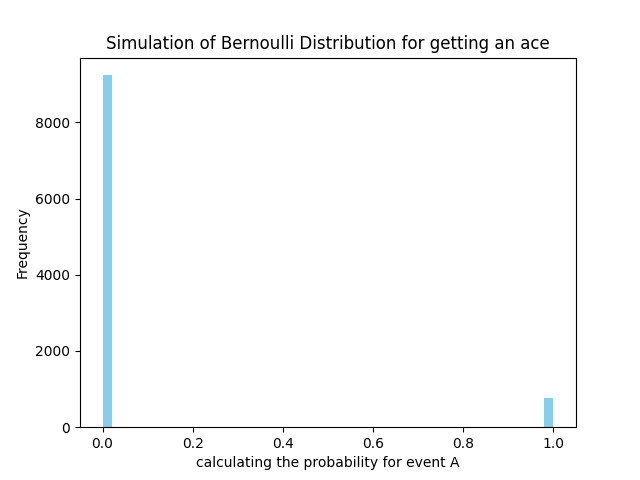
\includegraphics[width=\columnwidth] {Figure_1.png}

\end{figure}
\\

\end{document}

        

